{
\begin{figure*}[th]
\begin{minipage}{\figWidthSix}
\begin{center}
\centerline{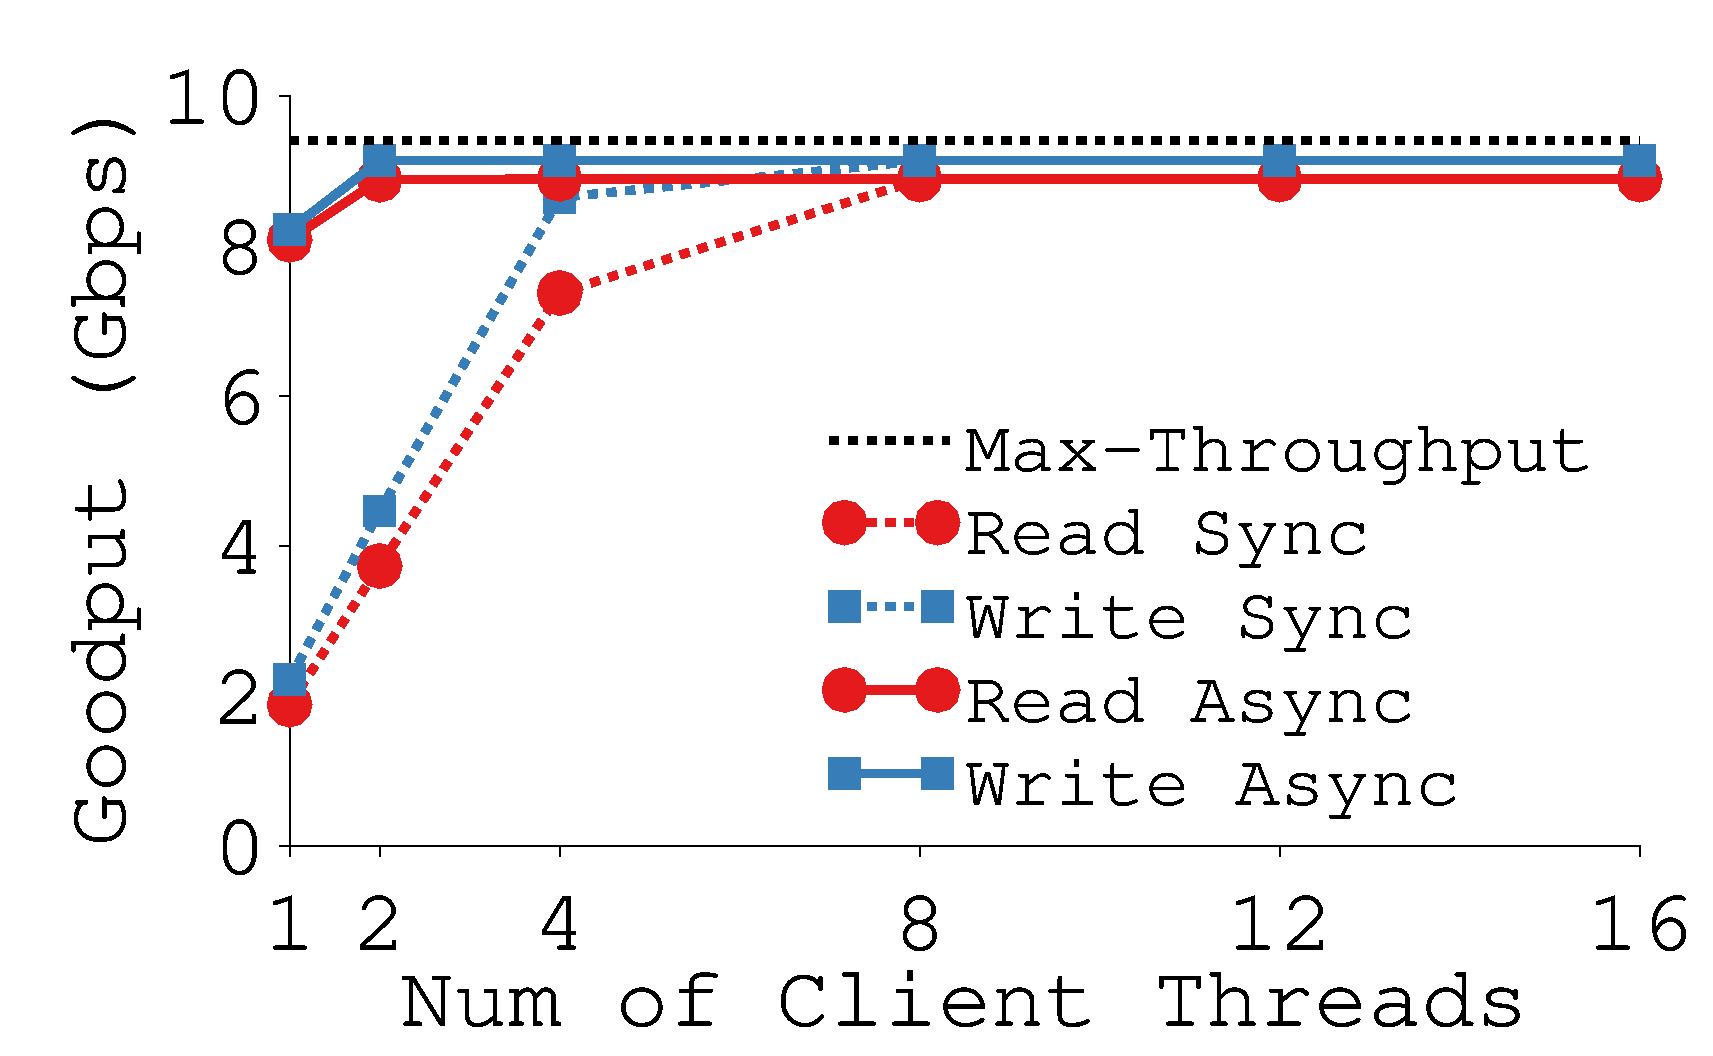
\includegraphics[width=\columnwidth]{Figures/g_plot_throughput.pdf}}
\vspace{-0.1in}
\captionsetup{width=.9\columnwidth}
\mycaption{fig-read-write-throughput}{End-to-End Goodput.}
{
1\KB\ requests. % between 1 \CN\ and 1 \MN.
}
\end{center}
\end{minipage}
\begin{minipage}{\figWidthSix}
\begin{center}
\centerline{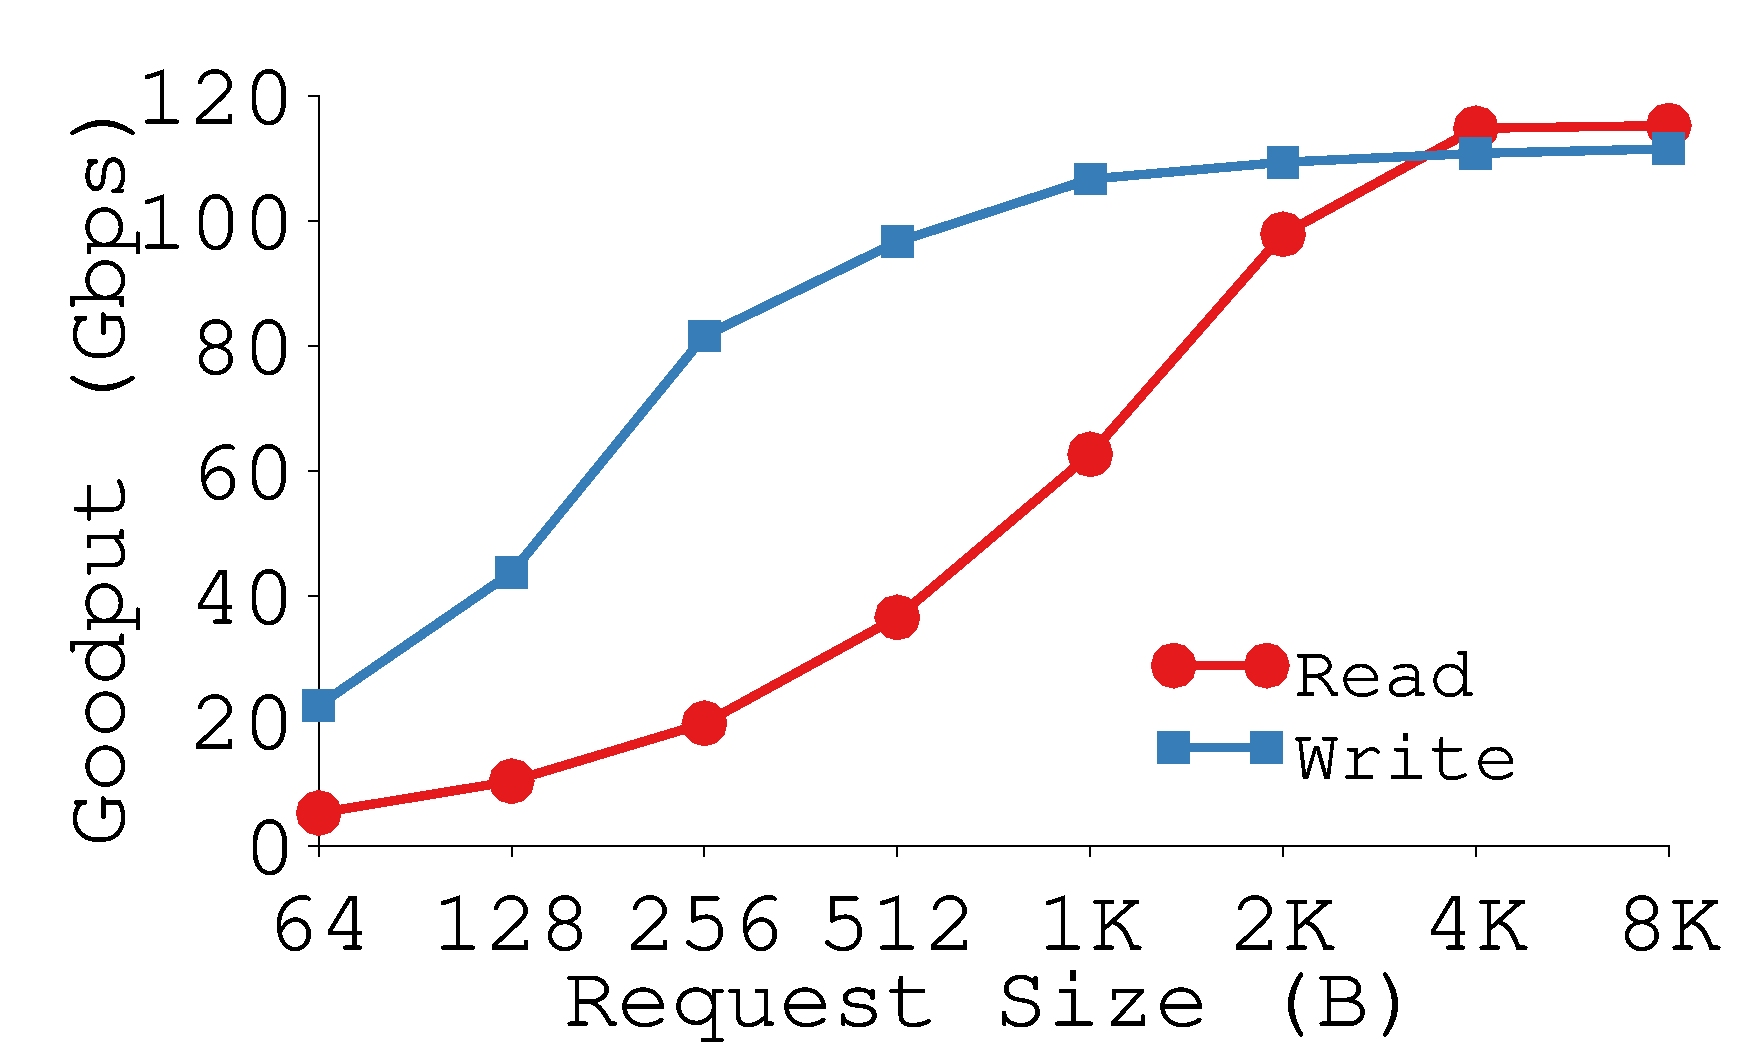
\includegraphics[width=\columnwidth]{Figures/g_plot_onboard_throughput.pdf}}
\vspace{-0.1in}
\captionsetup{width=.9\columnwidth}
\mycaption{fig-onboard-throughput}{On-board Goodput.}
{
FPGA test module generates requests at maximum speed.
}
\end{center}
\end{minipage}
\begin{minipage}{\figWidthSix}
\begin{center}
\centerline{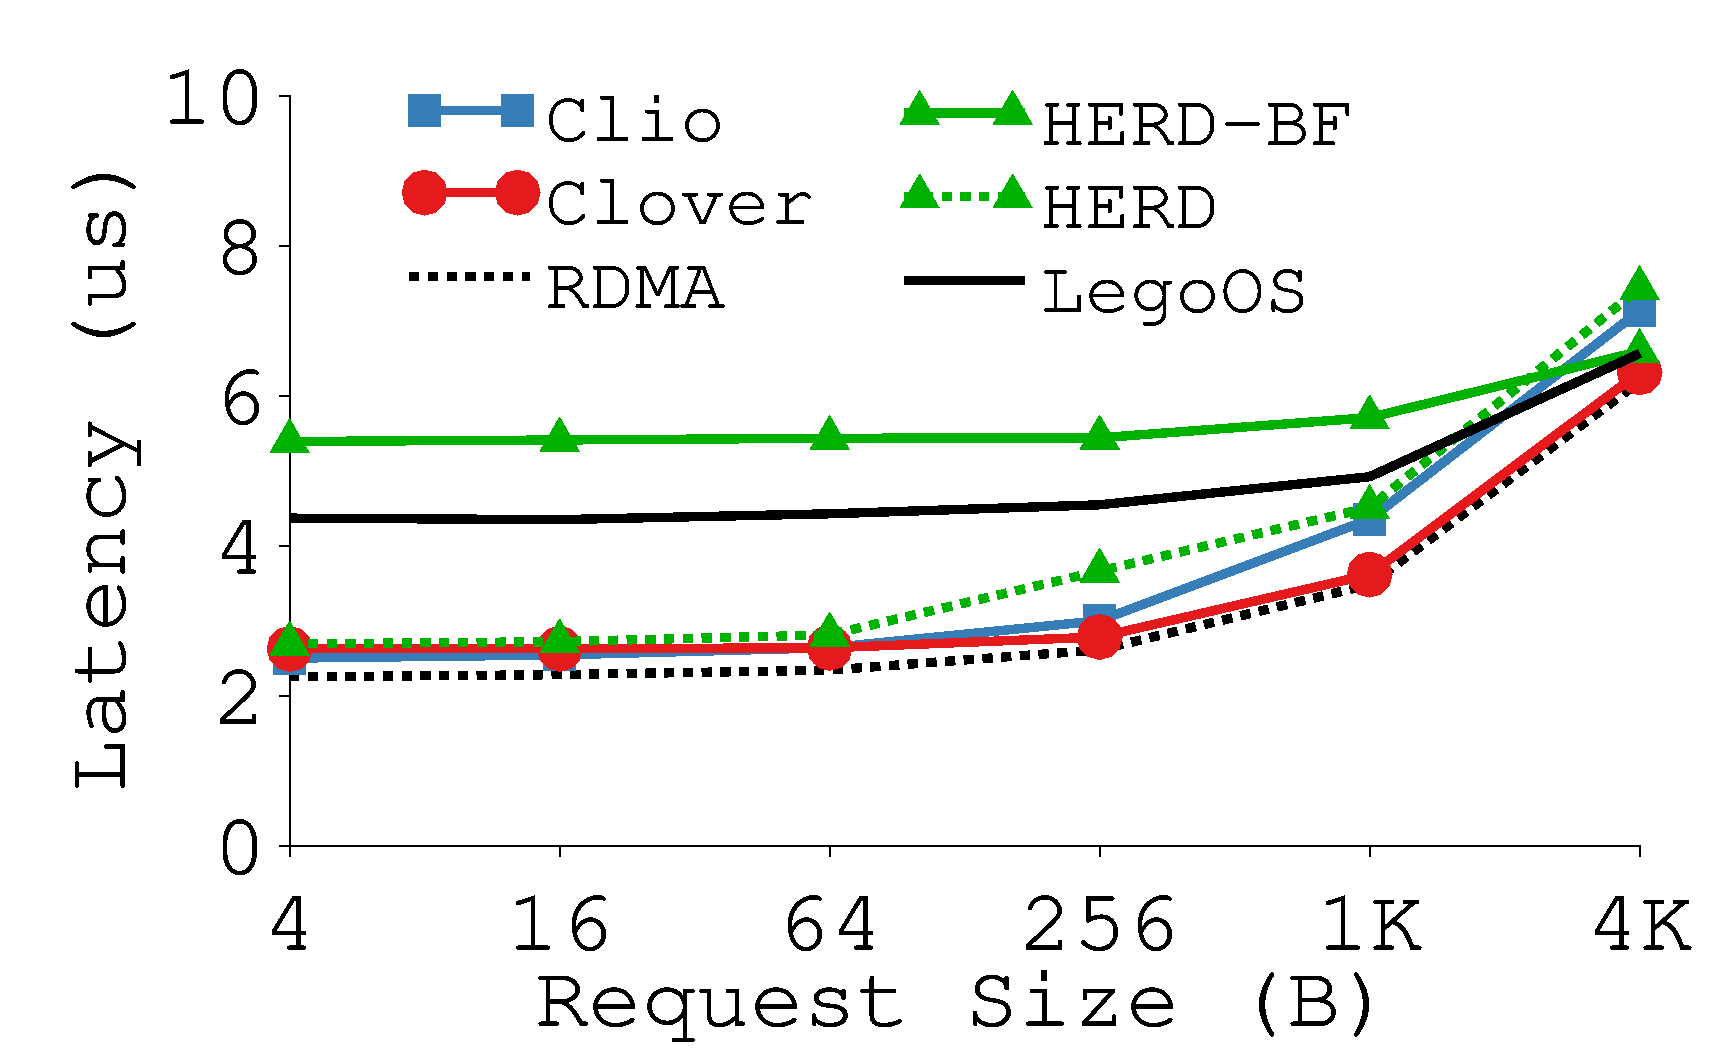
\includegraphics[width=\columnwidth]{Figures/g_plot_read_latency.pdf}}
\vspace{-0.1in}
\captionsetup{width=.9\columnwidth}
\mycaption{fig-read-lat}{Read Latency.}
{
HERD-BF: HERD running on BlueField. %SmartNIC.
}
\end{center}
\end{minipage}
\begin{minipage}{\figWidthSix}
\begin{center}
\centerline{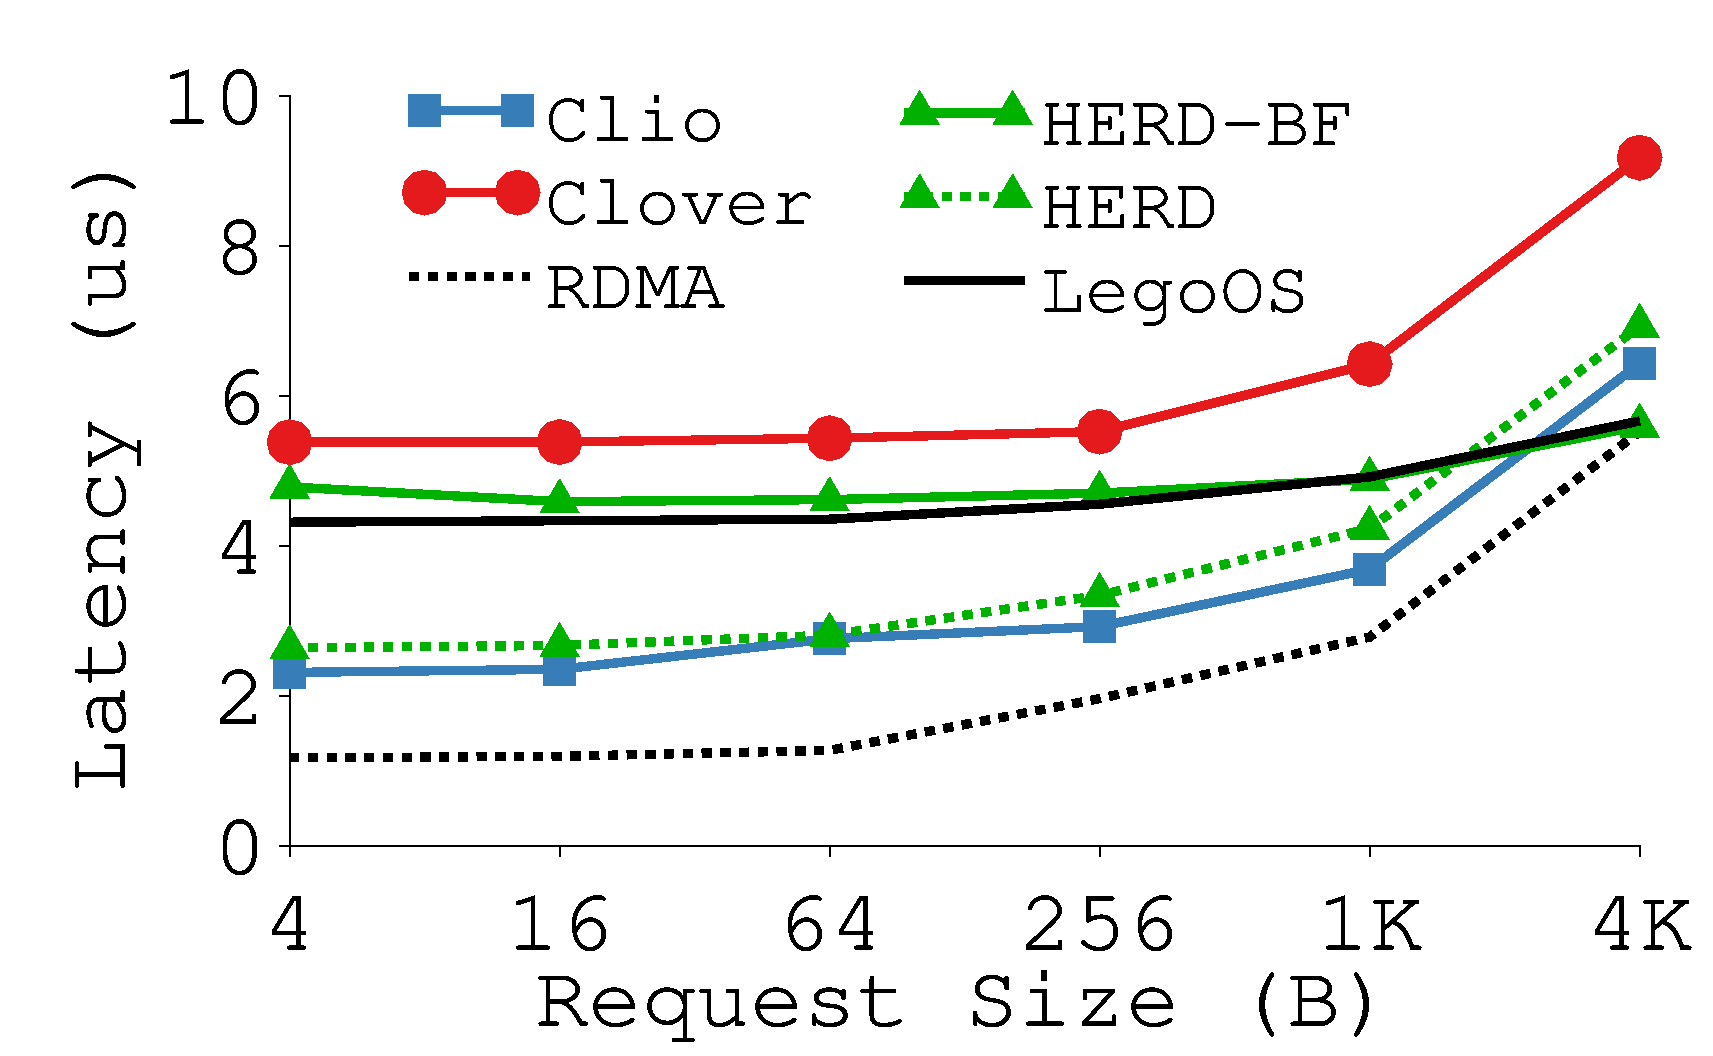
\includegraphics[width=\columnwidth]{Figures/g_plot_write_latency.pdf}}
\vspace{-0.1in}
\captionsetup{width=.9\columnwidth}
\mycaption{fig-write-lat}{Write Latency.}
{
Clover requires $\ge$ 2 RTTs for write.
}
\end{center}
\end{minipage}
%\vspace{-0.15in}
\end{figure*}
}
